\subsection{RQ1: Effectiveness of \tia on Real-world Chisel Designs}\label{sec:eval-tia}

We evaluate \tia's effectiveness along three complementary dimensions: recall, efficiency, and precision.
\emph{Recall} measures its ability to identify all temporal influences and serves as an empirical measure of its soundness;
\emph{efficiency} measures its computational cost;
\emph{precision} measures the proportion of reported temporal influences that are true.
These dimensions are widely used in empirical evaluations of static analyses~\cite{park_survey_2022,delaitre_sate_2018}.

\subsubsection{Experiment Design}\label{sec:exp-tia}

\paragraph{Benchmarks}
We selected 13 popular open-source Chisel hardware designs as real-world benchmarks, with an average of 2.2K GitHub stars.
These designs span diverse hardware domains, including system-on-chips (SoCs) with pipelined designs (\texttt{rocket}~\cite{asanovic_rocket_2016}, \texttt{quasar}~\cite{quasar}, 5 \texttt{sodor} designs~\cite{sodor}, and \texttt{riscv-mini}~\cite{riscvmini}) and superscalar designs (\texttt{boom}~\cite{celio_berkeley_2015} and \texttt{xiangshan}~\cite{xu_towards_2022}), a network-on-chip (NoC) design (\texttt{constellation}~\cite{zhao_constellation_2022}), a deep neural network (DNN) accelerator (\texttt{gemmini}~\cite{genc_gemmini_2021}), and a vector co-processor (\texttt{hwacha}~\cite{lee_hwacha_2015}).
These designs also diversely range from 2.7K to 4.0M LoC, with an average of 451.8K LoC, in pre-elaborated Firrtl~\cite{izraelevitz_reusability_2017}, the intermediate representation (IR) used by the Chisel compiler.
Their popularity, domain diversity, and wide range of sizes make them suitable for evaluating \tia's effectiveness on real-world hardware designs.

\paragraph{Ground Truth}
To empirically assess \tia's soundness and precision, we collect dynamic temporal influences from these real-world designs through \emph{runtime instrumentation}.
Specifically, for each input $p$ of a Chisel hardware design, we perturb the value of $p$ and simulate the design for 1,000 clock cycles for each clock.
If changing the value of $p$ causes the value of a variable $x$ to change at the $i$-th cycle after the perturbation, we record a \emph{temporal influence relation} $x \mapsto o_p^i$.
For a design with $m$ clocks and $n$ non-clock input ports, this process requires $m \times n \times 1000$ simulation cycles per run.
We repeat the process 10 times with different executions to improve coverage, resulting in a total of $m \times n \times 1000 \times 10$ simulation cycles for each design.
In total, we simulated 9,240,000 cycles for a total of 364h 17m 39s to collect these relations from the 13 real-world Chisel designs, achieving an average branch coverage of 86.8\%.
Note that even hundreds of hours of simulation cannot exhaustively exercise all possible executions and thus cannot collect all possible temporal influence relations.
The collected relations therefore constitute only a dynamic approximation---i.e., a subset---of the true ground truth.
Obtaining the true ground truth for the unbounded temporal behavior of these real-world hardware designs through finite runtime instrumentation is infeasible.
We therefore use the dynamically collected temporal influence relations as an approximation of the ground truth for evaluating \tia, following a common practice in empirical evaluations of static analyses~\cite{helm_total_2024,sui_recall_2020,liang_pointer_2025}.

\paragraph{Measures}
Given the dynamically collected temporal influence relations, denoted $\mathtt{dynamic}$, we calculate recall and precision to empirically assess \tia's soundness and precision as follows.
\emph{First}, we flatten \tia's result $\absT$ into temporal influence relations, denoted $\mathtt{static}$.
For example, if \tia's result is $\absT = \{x \mapsto \{o_p^0, o_p^1\}, y \mapsto \{o_p^2, o_q^2, o_r^0\}\}$, its flattened version is $\mathtt{static} = \{x \mapsto o_p^0, x \mapsto o_p^1, y \mapsto o_p^2, y \mapsto o_q^2, y \mapsto o_r^0\}$.
\emph{Second}, we compare $\mathtt{dynamic}$ and $\mathtt{static}$ to determine the dynamic temporal influence relations that are statically matched by \tia, denoted $\mathtt{match}$.
For example, given the above $\mathtt{static}$ and $\mathtt{dynamic} = \{x \mapsto o_p^0, x \mapsto o_p^3, y \mapsto o_p^2, y \mapsto o_q^2\}$, we have $\mathtt{match} = \mathtt{static} \cap \mathtt{dynamic} = \{x \mapsto o_p^0, y \mapsto o_p^2, y \mapsto o_q^2 \}$.
\emph{Third}, let $\mathtt{\#match}$, $\mathtt{\#dynamic}$, and $\mathtt{\#static}$ denote the numbers of temporal influence relations in the corresponding sets.
We define recall and precision as:
\begin{equation}\label{eq:recall-precision}
    \mathit{recall} = \frac{\mathtt{\#match}}{\mathtt{\#dynamic}}
    \quad
    \text{and}
    \quad
    \mathit{precision} = \frac{\mathtt{\#match}}{\mathtt{\#static}}.
\end{equation}
For the above example, we have $\mathit{recall} = \mathtt{\#match} / \mathtt{\#dynamic} = 3 / 4 = 75\%$ and $\mathit{precision} = \mathtt{\#match} / \mathtt{\#static} = 3 / 5 = 60\%$.

To obtain an informative measure of \tia's precision, we omit the portion of $\mathtt{static}$ beyond the runtime instrumentation bound (which is at most 1,000 clock cycles in our setup).
This treatment is necessary because all 13 real-world Chisel designs contain feedback loops that induce infinitely many temporal influences.
% TODO: as discussed in Section xxx
Without bounding the clock-cycle range of $\mathtt{static}$, we would always have $\mathtt{\#static} = \infty$, necessarily yielding a precision of $\mathtt{\#match}/\infty = 0$, which would provide no informative about \tia's precision.
Note that this bounding does not affect recall because recall depends only on $\mathtt{\#match}$ and $\mathtt{\#dynamic}$, neither of which is affected by the portion of $\mathtt{static}$ beyond the runtime instrumentation bound.

To measure \tia's efficiency, we simply record the wall-clock time spent by the analysis.

\subsubsection{Understanding the Results}

\begin{figure}[tp]
    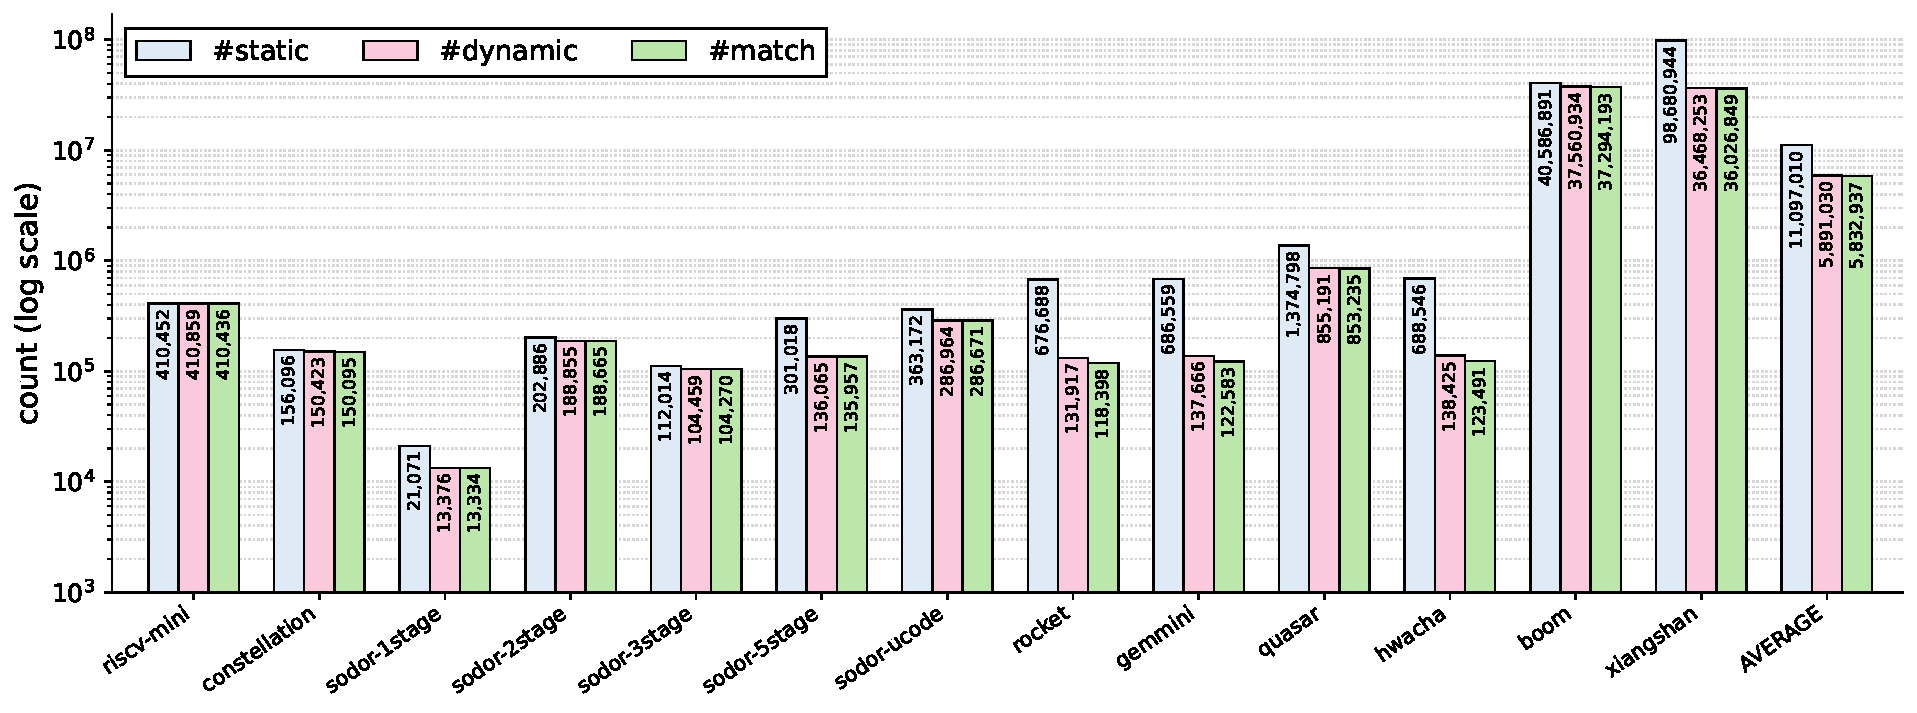
\includegraphics[width=\linewidth,clip,trim=8 10 15 12]{figures/tia-absolute-bars}
    \caption{\tia's results in revealing temporal influence relations in real-world Chisel designs.}\label{fig:tia-absolute}
\end{figure}


Figure~\ref{fig:tia-absolute} presents \tia's results in revealing temporal influence relations in real-world Chisel designs.
The absolute numbers of temporal influence relations captured by \tia (\texttt{\#static}), by runtime instrumentation (\texttt{\#dynamic}), and by both (\texttt{\#match}) are labeled on each bar.
The recall and precision calculated from the statistics in Figure~\ref{fig:tia-absolute} using Equation~\ref{eq:recall-precision} are presented in Figure~\ref{fig:tia-percent}.
Figure~\ref{fig:tia-percent} also presents the analysis time for each benchmark in the parentheses under the bars as an indication of \tia's efficiency.
Below, we separately detail \tia's soundness, precision, and efficiency based on these empirical results.

\begin{figure}[tp]
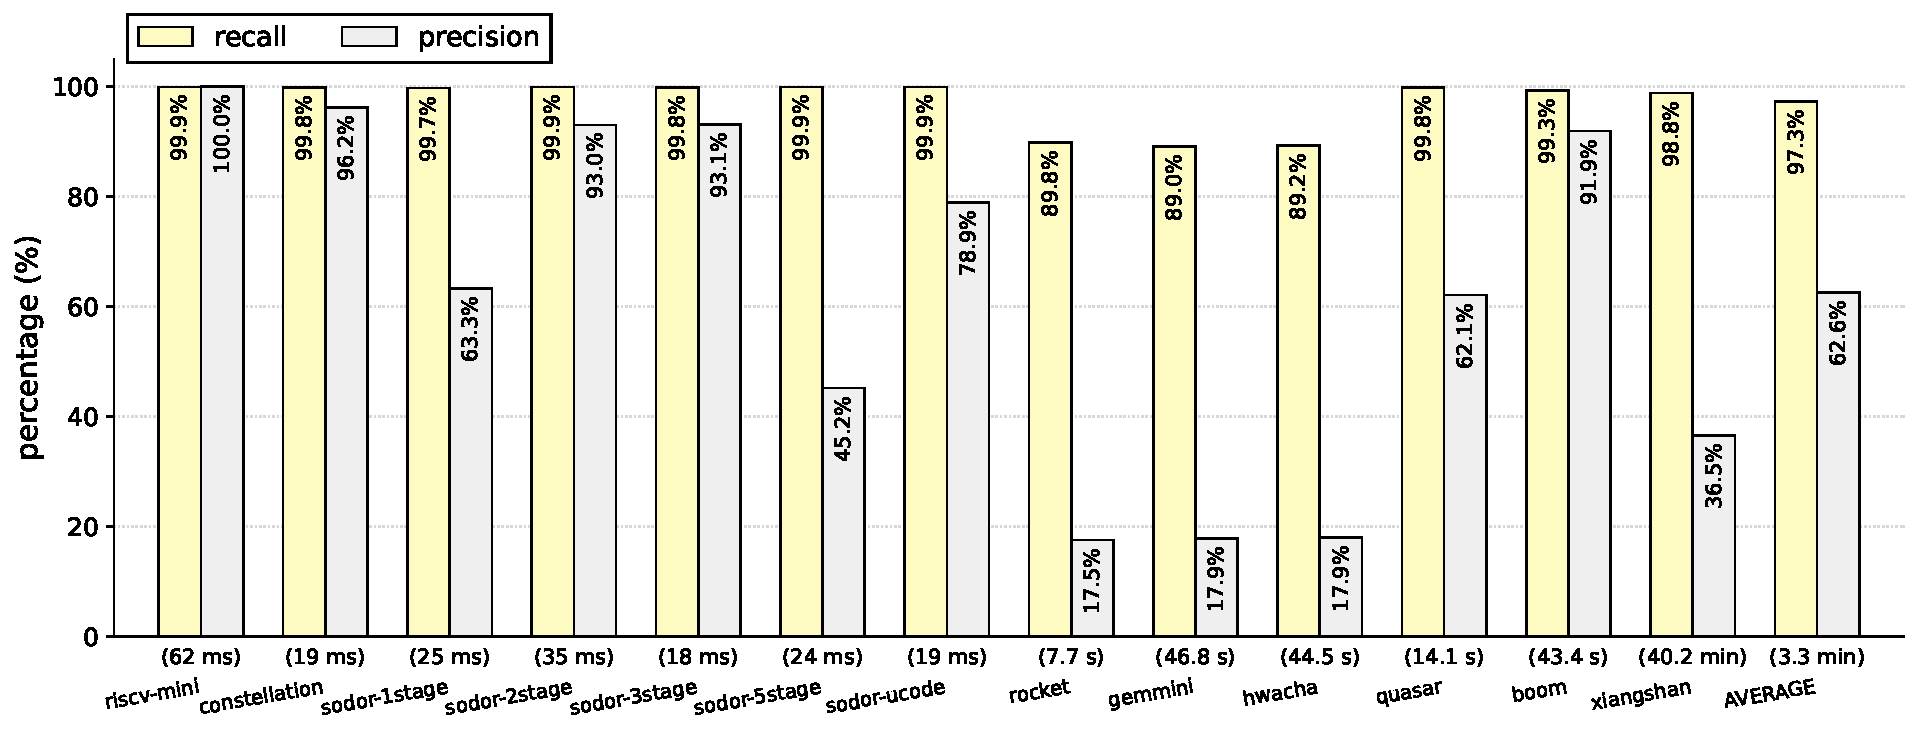
\includegraphics[width=\linewidth,clip,trim=8 9 18 5]{figures/tia-percent-bars}
\caption{Effectiveness of \tia on real-world Chisel designs, including recall (yellow bars), precision (gray bars), and efficiency (analysis time shown in parentheses under each bar).}\label{fig:tia-percent}
\end{figure}

\paragraph{Soundness}

\tia demonstrates strong empirical soundness, achieving an average recall of 97.3\%, as shown in the last column of Figure~\ref{fig:tia-percent}.
This high recall provides empirical evidence consistent with \tia's theoretical soundness. % TODO: in Theorems~\ref{theo:soundness} and~\ref{theo:}.
The small recall loss arises primarily from two limitations in handling complex real-world hardware designs.
(1) For external hardware modules whose source code is written in Verilog rather than Chisel, we model them as black boxes and assume a one-cycle delay between any input and output port.
This treatment is currently a heuristic engineering choice;
for example, the \texttt{plusarg\_reader} module in \texttt{rocket} cannot be soundly modeled using this heuristic.
Future work could investigate more systematic approaches, such as interactive static analysis across Chisel and Verilog.
(2) Since \tia's current theory focuses on synchronous hardware with a single global clock, for multiple-clock designs such as \texttt{hwacha} and \texttt{gemmini}, our implementation applies \tia rules independently to each clock domain as an engineering approximation.
This treatment may miss subtle temporal behaviors involving clock-domain crossings (CDCs)~\cite{chong_clock_2021}.
Future work could extend \tia's theory to multi-clock designs by explicitly tracking temporal influences with respect to each clock and developing rules for temporal interactions across clock domains.

\paragraph{Precision}
As the first static analysis primarily designed to soundly reason about infinite temporal influences in hardware designs, \tia achieves reasonable precision, with an average precision of 62.6\%, as shown in the last column of Figure~\ref{fig:tia-percent}.
This measured precision is an under-estimation of \tia's actual precision because we evaluate against only a subset of the true ground truth obtained through runtime instrumentation;
temporal influences reported by \tia but not observed dynamically may correspond to true influences that were simply not exercised during simulation.
Beyond this inherent under-estimation, we observe two major sources of imprecision in \tia.
\emph{(1) Memory Cell Insensitivity.}
For efficiency, we currently abstract an entire memory as a single abstract memory cell when analyzing memory accesses.
This coarse-grained abstraction can merge distinct temporal influence flows when they propagate through the memory, introducing false positives.
For example, the largest Chisel memory in \texttt{rocket} contains 16,384 cells, all of which are merged into a single abstract memory cell.
Although this abstraction is sound, it can introduce substantial imprecision.
A finer-grained memory abstraction could alleviate this problem and constitutes a direction for future work.
\emph{(2) Path Insensitivity.}
We currently soundly assume that the condition of each multiplexer (analogous to an \texttt{if}-statement in software) can evaluate to either true or false.
This path-insensitive treatment can introduce false positives.
For example, the conditions $a$ and $\neg a$ cannot both be true or both be false simultaneously, but our current analysis cannot exploit this mutual exclusivity to eliminate the corresponding false positives.
Introducing path sensitivity in the future could therefore further improve \tia's precision.


\paragraph{Efficiency}

As shown in Figure~\ref{fig:tia-percent}, \tia analyzes the 13 real-world hardware designs, totaling 5.9M LoC, in 42.8 minutes in total, 510.7$\times$ faster the 364.3 hours required by dynamic runtime instrumentation while achieving an average recall of 97.3\% in capturing dynamically observed temporal influences.
This result demonstrates the efficiency advantage of static analysis over simulation-based approaches for analyzing real-world hardware designs containing millions of lines of code.
The slowest case is \texttt{xiangshan}, which takes 40.2 minutes to analyze due to its large size of 4.0M LoC, yet remains substantially more efficient than dynamic simulation.

